\documentclass[11pt]{article}

\usepackage{lscape}

\usepackage{graphicx}
\usepackage[utf8]{inputenc}
\begin{document}
\begin{landscape}

\begin{minipage}{0.45\textwidth}
\underline{\textbf{Grundformeln}}\\
WS: $R = \frac{U}{I} = \frac{\rho * l}{A}$; $[R] = 1\frac{V}{A} =1 \Omega$ \\
Leitwert: $G = \frac{1}{R}$\\
Maschensatz: $\sum U_i = 0$\\
Knotensatz: $\sum I_i = 0$\\
Reihe WS: $R_{ges} = \sum R_i$\\
Parallel WS: $\frac{1}{R_ges} = \sum \frac{1}{R_i}$\\
\phantom{ss} Spezialfall: $R_{ges} = \frac{R_1 * R_2}{R1+R2} $\\
Spannungs-Teiler: $\frac{U_1}{U_2} = \frac{R_1}{R_2}$\\
Strom-Teiler: $\frac{I_1}{I_2} = \frac{R_2}{R_1}$\\
Leistung: $P =U*I = \frac{U^2}{R} = I^2*R $ \\
\phantom{ssssssssss} $[P] = 1V*A =1 W$\\
\underline{\textbf{Kondensator:}}\\
Kapazität: $C = \frac{Q}{U}, [C]=1F$\\
Kond. in Reihe: $Q_1 = Q_2 = Q_{12}$\\
Stromdichte: $S=\frac{I}{A}$\\
Feldstärke: $E=\frac{S}{\kappa}$\\
Spannungsabfall: $U=E*l$\\
Potenzial: $\varphi = \int_x^0 E(s)ds + \varphi(0)$\\
%TODO 2.4
$\tau = R*C$\\
Zeit Auf-/Entlanden: $t = 3\tau$\\
\underline{\textbf{Leitungen:}}\\
$k_0 = \frac{R_w}{R_w + R_i} $\\
$r_a = \frac{R_a - R_w}{R_a + R_w} $\\
$k_a = 1 + r_a$\\
Anfang: $U_k(0,t)=k_0*U_{q1}(t)$\\
Ende: $U_k(x,t)= k_0*U_{q1}(t-\Delta t)$
Auskoppeln Gatter:\\
\phantom{ss} $U_1(t) = k_a * U_1(x,t)$\\
$\Delta t = l/c$\\
%Aufladen über WS: $
\end{minipage}%
~~~~~~~
\begin{minipage}{0.3\textwidth}
\underline{\textbf{Koaxialkabel}}:\\
$R_W = \sqrt{\frac{L'}{C'}}$\\
    \phantom{sssi} $=\frac{\sqrt{\epsilon_R * \mu_R}}{c_0 * C'}$\\
    \phantom{sssi} $=\frac{\sqrt{\mu_R} * ln(\frac{d_a}{d_i})}{2c_0 * \pi * \epsilon_0 *\sqrt{\epsilon_R}}$\\
\underline{\textbf{Operationsverstärker}}:\\
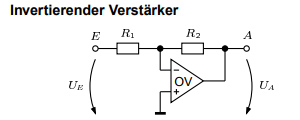
\includegraphics[scale=0.40]{IOV.png}
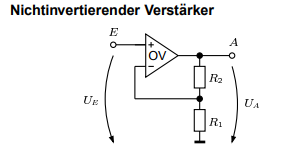
\includegraphics[scale=0.40]{NIOV.png}
$U_D = 0$
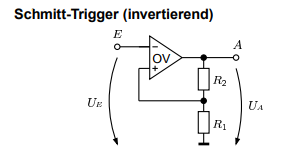
\includegraphics[scale=0.40]{ISTOV.png}
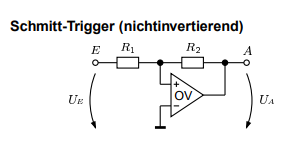
\includegraphics[scale=0.40]{NISTOV.png}
% TODO U_D = ?

\end{minipage}%
~~~~~~
\begin{minipage}{0.3\textwidth}
3. Spalte
\end{minipage}%

\end{landscape}
\end{document}
